% ---------------------------------------------------------------
% Cartoon macros (colours match the plots)
\definecolor{cBlue}{HTML}{257DE0}\definecolor{cOrange}{HTML}{F47230}
\definecolor{cAqua}{HTML}{00B894}\definecolor{cViolet}{HTML}{6A4CE2}
\definecolor{cGray}{HTML}{666666}\definecolor{cDark}{HTML}{191919}
\tikzset{
  gate/.style={draw=cBlue, fill=cBlue!10, rounded corners=2pt, font=\small, inner sep=1pt},
  hgate/.style={draw=cViolet, fill=cViolet!10, rounded corners=2pt, font=\small, inner sep=1pt},
  noise/.style={draw=cOrange, fill=cOrange!15, rounded corners=1pt, font=\scriptsize, inner sep=1.5pt},
  ewire/.style={line width=2.4pt, cGray!45},
  swire/.style={thick, cDark},
  lab/.style={font=\footnotesize, text=cDark},
  small/.style={font=\scriptsize, text=cGray},
}
\newcommand{\meter}[2]{%
  \draw[fill=white, rounded corners=1pt] ($#1+(-0.2,-0.15)$) rectangle ($#1+(0.2,0.15)$);
  \draw ($#1+(-0.12,-0.07)$) arc (160:20:0.13);
  \draw[-{Stealth[length=2pt]}] ($#1+(0,-0.09)$) -- ($#1+(0.09,0.09)$);
  \node[font=\scriptsize, above] at ($#1+(0,0.14)$) {#2};}
% ---------------------------------------------------------------

\newcommand{\CartoonModelOne}{%
\begin{figure}[!htbp]
\centering
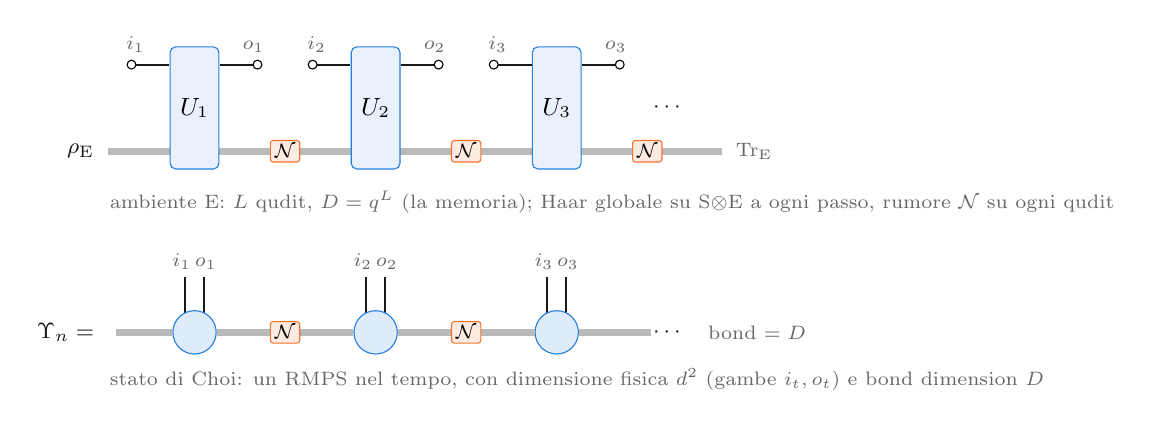
\begin{tikzpicture}[x=1cm, y=1cm]
  % ----- circuit
  \node[lab, anchor=east] at (-0.55,0) {$\rho_{\rm E}$};
  \draw[ewire] (-0.5,0) -- (7.3,0);
  \node[small, anchor=west] at (7.35,0) {$\mathrm{Tr}_{\rm E}$};
  \foreach \i/\x in {1/0.6, 2/2.9, 3/5.2} {
    \draw[swire] (\x-0.8,1.1) -- (\x-0.32,1.1); \draw[fill=white] (\x-0.8,1.1) circle (1.6pt);
    \node[small, above] at (\x-0.75,1.13) {$i_{\i}$};
    \draw[swire] (\x+0.32,1.1) -- (\x+0.8,1.1); \draw[fill=white] (\x+0.8,1.1) circle (1.6pt);
    \node[small, above] at (\x+0.75,1.13) {$o_{\i}$};
    \node[gate, minimum width=0.62cm, minimum height=1.55cm] at (\x,0.55) {$U_{\i}$};
    \node[noise] at (\x+1.15,0) {$\mathcal N$};
  }
  \node[lab] at (6.6,0.55) {$\cdots$};
  \node[small, align=left, anchor=west] at (-0.6,-0.65) {ambiente E: $L$ qudit, $D=q^L$ (la memoria); Haar globale su S$\otimes$E a ogni passo, rumore $\mathcal N$ su ogni qudit};
  % ----- MPS in time
  \begin{scope}[yshift=-2.3cm]
    \node[lab, anchor=east] at (-0.55,0) {$\Upsilon_n=$};
    \foreach \i/\x in {1/0.6, 2/2.9, 3/5.2} {
      \draw[swire] (\x-0.12,0.15) -- (\x-0.12,0.7); \draw[swire] (\x+0.12,0.15) -- (\x+0.12,0.7);
      \node[small, above] at (\x,0.68) {$i_{\i}\,o_{\i}$};
      \node[circle, draw=cBlue, fill=cBlue!15, minimum size=0.55cm, inner sep=0pt] (T\i) at (\x,0) {};
    }
    \draw[ewire] (-0.4,0) -- (T1); \draw[ewire] (T1) -- (T2); \draw[ewire] (T2) -- (T3); \draw[ewire] (T3) -- (6.4,0);
    \foreach \x in {1.75, 4.05} {\node[noise] at (\x,0) {$\mathcal N$};}
    \node[lab] at (6.6,0) {$\cdots$};
    \node[small, anchor=west] at (7.0,0) {bond $=D$};
    \node[small, anchor=west] at (-0.6,-0.6) {stato di Choi: un RMPS nel tempo, con dimensione fisica $d^2$ (gambe $i_t,o_t$) e bond dimension $D$};
  \end{scope}
\end{tikzpicture}
\caption{Modello 1. In alto: il circuito di collisione con memoria. Le gambe aperte $i_t$ (ingresso) e $o_t$ (uscita) di S sono quelle di Choi, e il rumore $\mathcal N$ agisce sull'ambiente fra un passo e l'altro. In basso: il process tensor $\Upsilon_n$ è un MPS nel tempo il cui legame è l'ambiente; il rumore agisce sui legami.}
\label{fig:cartoon-m1}
\end{figure}}

\newcommand{\CartoonReplica}{%
\begin{figure}[!htbp]
\centering
\begin{tikzpicture}[x=1cm, y=1cm]
  % ----- identity label (box)
  \begin{scope}[shift={(0,0)}]
    \draw[ewire, cBlue!60] (0,0.35) -- (1.4,0.35); \draw[ewire, cBlue!60] (0,-0.35) -- (1.4,-0.35);
    \node[small, anchor=east] at (0,0.35) {1}; \node[small, anchor=east] at (0,-0.35) {2};
    \node[lab] at (0.7,-0.95) {$\square$: ogni replica};
    \node[lab] at (0.7,-1.3) {tracciata da sé};
  \end{scope}
  % ----- swap label (circle)
  \begin{scope}[shift={(4.4,0)}]
    \draw[ewire, cOrange!70] (0,0.35) .. controls (0.7,0.35) and (0.7,-0.35) .. (1.4,-0.35);
    \draw[ewire, cOrange!70] (0,-0.35) .. controls (0.7,-0.35) and (0.7,0.35) .. (1.4,0.35);
    \node[small, anchor=east] at (0,0.35) {1}; \node[small, anchor=east] at (0,-0.35) {2};
    \node[lab] at (0.7,-0.95) {$\circ$: repliche legate};
    \node[lab] at (0.7,-1.3) {(memoria / eco)};
  \end{scope}
  % ----- transitions
  \draw[-{Stealth[length=5pt]}, thick, cDark] (1.8,0.65) to[out=120, in=60, looseness=4] node[above, lab] {$a\simeq1/d^2$} (2.1,0.65);
  \draw[-{Stealth[length=5pt]}, thick, cDark] (4.25,0.65) to[out=120, in=60, looseness=4] node[above, lab] {$u_{\rm eff}\simeq(g_F/q^2)^L$} (4.55,0.65);
  \draw[-{Stealth[length=5pt]}, thick, cOrange] (4.1,-0.1) -- node[below, lab, text=cOrange] {rumore} (2.0,-0.1);
  % ----- level crossing inset
  \begin{scope}[shift={(7.6,-1.2)}]
    \draw[-{Stealth[length=4pt]}, cGray] (0,0) -- (3.0,0) node[right, small] {$L$};
    \draw[-{Stealth[length=4pt]}, cGray] (0,0) -- (0,2.1) node[above, small] {autovalori};
    \draw[thick, cBlue] (0,0.9) -- (2.8,0.9) node[right, small, text=cBlue] {Markov};
    \draw[thick, cOrange] (0,1.9) .. controls (1.0,1.2) and (1.8,0.6) .. (2.8,0.25) node[right, small, text=cOrange] {memoria};
    \draw[dashed, cGray] (1.32,0) -- (1.32,0.9); \node[small, below] at (1.32,0) {$L^*$};
  \end{scope}
\end{tikzpicture}
\caption{Struttura a due repliche, comune ai due modelli. L'ambiente porta un'etichetta: $\square$ (identità) o $\circ$ (scambio delle repliche). Il rumore agisce replica per replica e quindi smorza solo $\circ$. Nel modello 1 il settore di memoria decade come $(g_F/q^2)^L$ e incrocia il settore Markoviano ($a\simeq1/d^2$) in $L^*$: oltre l'incrocio la memoria crolla.}
\label{fig:cartoon-replica}
\end{figure}}

\newcommand{\CartoonModelTwo}{%
\begin{figure}[!htbp]
\centering
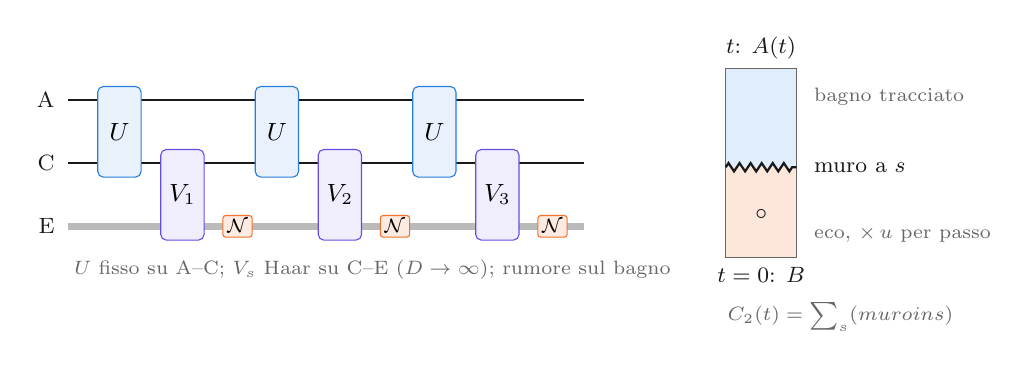
\begin{tikzpicture}[x=1cm, y=1cm]
  % ----- circuit A, C, E
  \node[lab, anchor=east] at (-0.3,1.6) {A}; \node[lab, anchor=east] at (-0.3,0.8) {C}; \node[lab, anchor=east] at (-0.3,0) {E};
  \draw[swire] (-0.25,1.6) -- (6.3,1.6); \draw[swire] (-0.25,0.8) -- (6.3,0.8); \draw[ewire] (-0.25,0) -- (6.3,0);
  \foreach \i/\x in {1/0.4, 2/2.4, 3/4.4} {
    \node[gate, minimum width=0.55cm, minimum height=1.15cm] at (\x,1.2) {$U$};
    \node[hgate, minimum width=0.55cm, minimum height=1.15cm] at (\x+0.8,0.4) {$V_{\i}$};
    \node[noise] at (\x+1.5,0) {$\mathcal N$};
  }
  \node[small, anchor=west] at (-0.3,-0.55) {$U$ fisso su A--C; $V_s$ Haar su C--E ($D\to\infty$); rumore sul bagno};
  % ----- replica contour with domain wall
  \begin{scope}[shift={(8.1,-0.4)}]
    \fill[cOrange!18] (0,0) rectangle (0.9,1.15);
    \fill[cBlue!14] (0,1.15) rectangle (0.9,2.4);
    \draw[cGray] (0,0) rectangle (0.9,2.4);
    \draw[thick, cDark, decorate, decoration={zigzag, segment length=4pt, amplitude=1.5pt}] (0,1.15) -- (0.9,1.15);
    \node[lab, anchor=west] at (1.0,1.15) {muro a $s$};
    \node[lab] at (0.45,0.55) {$\circ$}; \node[lab] at (0.45,1.8) {$\square$};
    \node[small, anchor=west] at (1.0,0.3) {eco, $\times\,u$ per passo};
    \node[small, anchor=west] at (1.0,2.05) {bagno tracciato};
    \node[lab, below] at (0.45,0) {$t=0$: $B$};
    \node[lab, above] at (0.45,2.4) {$t$: $A(t)$};
    \node[small, anchor=west] at (-0.1,-0.75) {$C_2(t)=\sum_s(\text{muro in }s)$};
  \end{scope}
\end{tikzpicture}
\caption{Modello 2. A sinistra: il bagno a collo di bottiglia, con il sistema A, il sito C e il bagno E. A destra: a due repliche e $D=\infty$ l'OTOC è una somma sulla posizione $s$ di un muro di dominio. Sotto il muro c'è il settore dell'eco $\circ$, che il rumore sul bagno smorza di $u=(1-p)^2$ a ogni passo; sopra c'è il settore $\square$, che il rumore non tocca.}
\label{fig:cartoon-m2}
\end{figure}}

\newcommand{\CartoonIPR}{%
\begin{figure}[!htbp]
\centering
\begin{tikzpicture}[x=1cm, y=1cm]
  \node[lab, anchor=east] at (-0.3,1.0) {S}; \node[lab, anchor=east] at (-0.3,0) {E};
  \draw[ewire] (-0.25,0) -- (6.0,0);
  \draw[swire] (-0.25,1.0) -- (6.0,1.0);
  \foreach \i/\x/\b in {1/0.4/0, 2/1.9/1, 3/3.4/1, 4/4.9/0} {
    \node[gate, minimum width=0.5cm, minimum height=1.35cm] at (\x,0.5) {$U_{\i}$};
    \meter{(\x+0.68,1.0)}{$o_{\i}=\b$}
  }
  \node[lab] at (6.35,0.5) {$\cdots$};
  \node[lab, anchor=west] at (-0.3,-0.75) {record $x=(0,1,1,0,\dots)\ \Rightarrow\ p(x),\ \mathcal I_2=\sum_x p(x)^2$};
  % ----- distributions
  \begin{scope}[shift={(8.0,-0.2)}]
    \draw[-{Stealth[length=4pt]}, cGray] (-0.2,0) -- (3.6,0) node[right, small] {$\ln Np$};
    \draw[thick, cBlue, domain=1.2:2.6, samples=60] plot (\x, {1.9*exp(-((\x-1.9)^2)/0.03)});
    \draw[thick, cOrange, domain=-0.1:3.4, samples=80] plot (\x, {0.65*exp(-((\x-1.5)^2)/0.6)});
    \node[small, text=cBlue, anchor=west] at (2.05,1.7) {$n\ll D$: quasi uniforme};
    \node[small, text=cOrange, anchor=west] at (2.3,0.75) {$n\gg D$: log-normale};
    \draw[dashed, cGray] (1.9,0) -- (1.9,2.05);
  \end{scope}
\end{tikzpicture}
\caption{IPR temporale. La sonda S viene misurata dopo ogni passo e la sua storia di esiti è il record $x$. A destra: la distribuzione di $\ln(Np)$ è log-normale. È stretta (record quasi uniformi) finché $n\ll D$, poi si allarga con varianza $(1-1/d)\,n/D$.}
\label{fig:cartoon-ipr}
\end{figure}}
